%!TEX root = ../tesis.tex
\chapter{Desarrollo de la Ontología}
\label{chap:Desarrollo de la Ontologia}

Luego de haber estudiado las distintas metodologías para el desarrollo de ontologías, se decidió utilizar la metodología NeOn, ya que la misma según la tabla xx posee mayor especificación en las actividades a desarrollar  y contempla los caso de reuso de recursos ontológicos y no-ontológicos. 

Siguiendo la metodología NeOn se identifica que la ontología a desarrollar sigue las actividades compuestas principalmente por los escenarios 1, 2 y 3 que se exponen de la metodología. El escenario 1, puesto que se quiere modelar una ontología desde el principio y es la base de los demás escenarios, el escenario 2 y 3 ya que se pretende reusar recursos ontológicos y no-ontológicos. A continuación se detalla la primera actividad que consiste en la especificación de los requerimiento de la ontología.


\section{Especificación de requerimientos de la ontología}

En esta actividad se define el alcance y los requerimientos de la ontología a desarrollar. Como resultado de esta actividad se obtiene el Documento de Especificación de Requerimientos de la Ontología (ORSD). A continuación se detalla el resultado de dicho proceso.
\begin{enumerate}
\item \textbf{Propósito:} Crear una ontología para el dominio de Contrataciones Públicas para lograr la interoperabilidad semántica con otras fuentes de datos externas utilizando el OCDS como base de conocimiento principal aumentando la formalidad semántica como se muestra en la figura \ref{img:ocds-ocntology-complejidad}

\begin{figure}[h!]
\centering
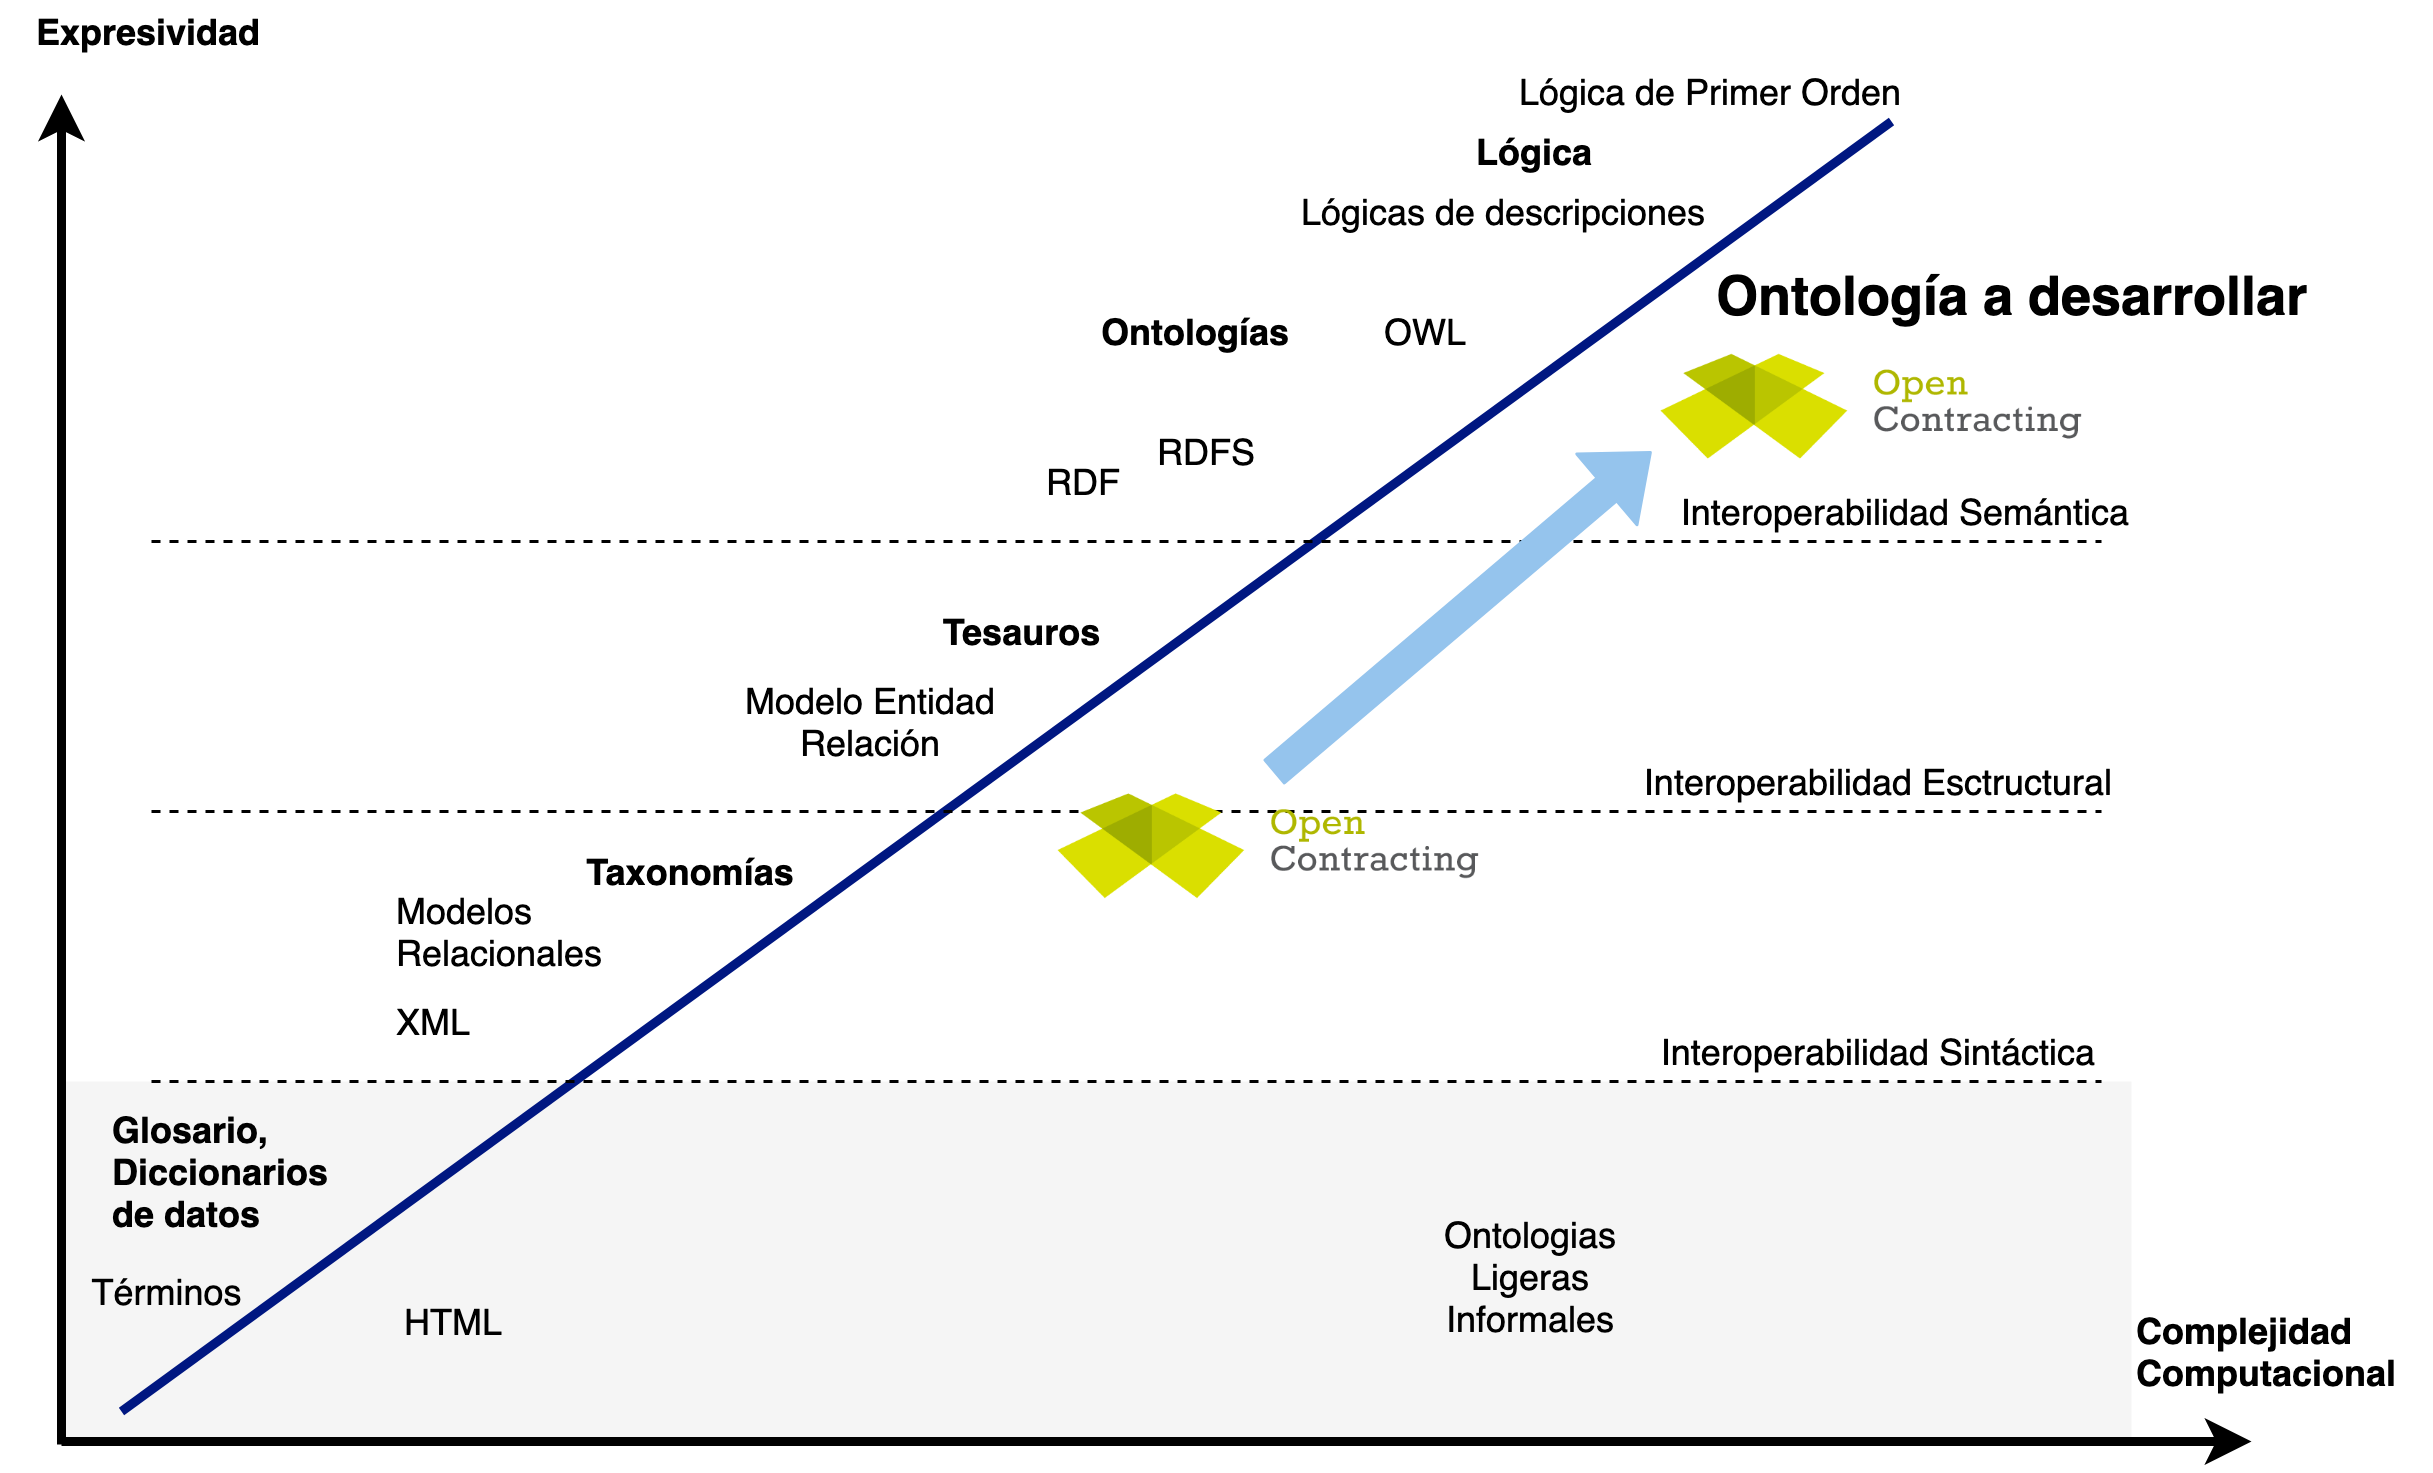
\includegraphics[width=150mm]{figuras/Diagramas-OenContracting.png}
\caption{Nivel de complejidad semántica de la ontología a desarrollar}
\label{img:ocds-ocntology-complejidad}
\end{figure}
\item \textbf{Alcance:} El alcance de la ontología está delimitada por el vocabulario detallado en la versión 1 del OCDS. Ya que en el momento del inicio de esta investigación era la última versión estable del estándar.
\item \textbf{Lenguaje de Implementación.} Se utilizará el lenguaje OWL debido a que es el lenguaje preferido para ontologías en la web semántica recomendado por la W3C, y se requiere de una ontología lo suficientemente ligera y explícita que se pueda manejar en la web semántica.
\item \textbf{Grupo Objetivo. }La ontología está orientada a:
\begin{enumerate}
    \item Expertos del dominio de Contrataciones Públicas que quieran realizar consultas ad-hoc sobre datos.
    \item Desarrolladores de software que deseen implementar el OCDS.
    \item Desarrolladores de software que necesiten integrar datos de contrataciones públicas con otras fuentes externas. \end{enumerate}
\item \textbf{Usos de la Ontología. }La ontología se utilizará para crear un esquema de publicación en JSON-LD, esto es debido a que la sintaxis JSON es ampliamente conocida y preferida por los desarrolladores, además el OCDS ya posee un esquema de publicación compatible con esta sintaxis. Los datos utilizados se extraerán del portal de datos abiertos de la DNCP.
\item \textbf{Requerimientos No Funcionales: }
\begin{enumerate}
    \item Se optará, en lo posible, por la reutilización de otras ontologías del dominio de Contrataciones Públicas ampliamente utilizadas.
    \item La ontología desarrollada debe ser procesable dentro de las limitaciones de la web semántica, ósea debe ser una ontología ligera.
    \item Debe soportar múltiples lenguajes: inglés y español inicialmente.
\end{enumerate}
\item \textbf{Requerimientos Funcionales. }
    \begin{enumerate}
        \item Gracias a la ontología se podrán responder las mismas preguntas que se responden a través de los datos publicados en formato de JSON y se podrán responder preguntas de todas las fases del proceso licitatorio.
        \item Debe ser compatible con la versión 1 del OCDS.
        \item Los datos deberán poder ser enriquecidos con otras fuentes de datos provenientes de la DNCP y también fuentes externas como Wikidata o DBpedia.
    \end{enumerate}
\item \textbf{Pre-Glosario de Términos.} El glosario fue extraído del diccionario de datos y de la ontología desarrollada por la DNCP. 
\end{enumerate}

\begin{figure}[h!]
    \centering
    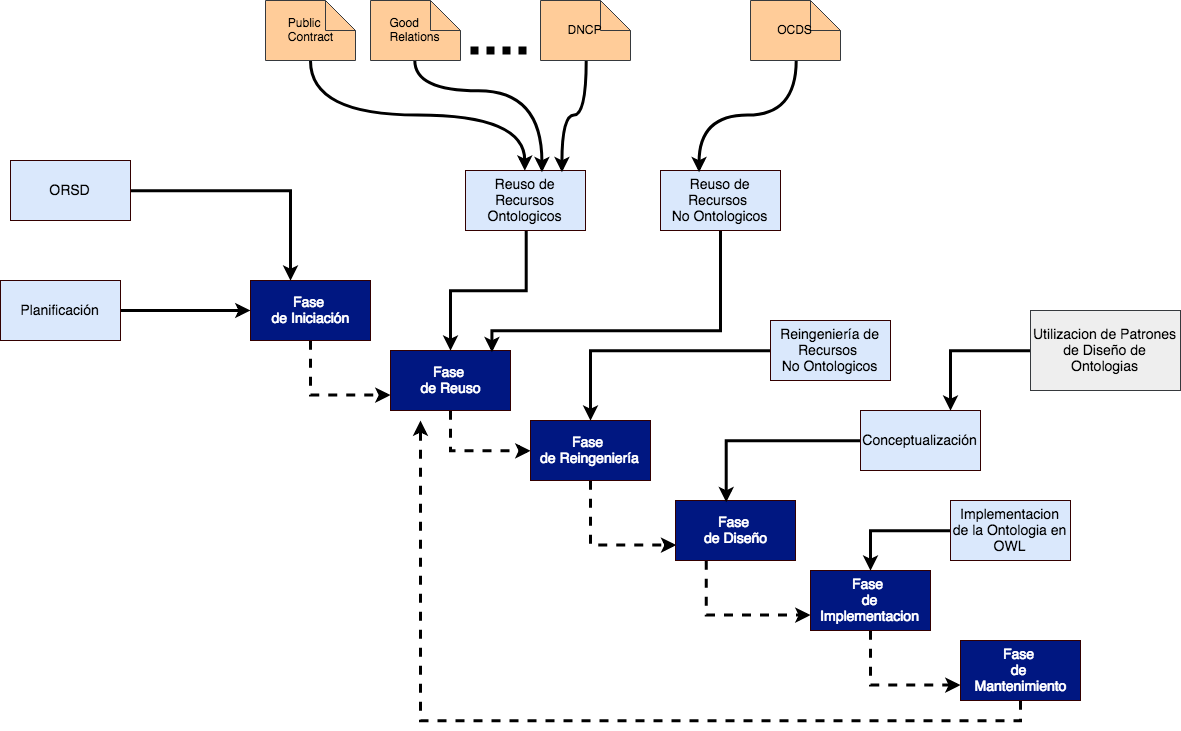
\includegraphics[width=150mm]{figuras/Diagramas-Grafico de Secuencias Desarrollo.png}
    \caption{Modelo de ciclo de vida de desarrollo de la ontología a desarrollar}
    \label{img:secuencia de desarrollo}
    \end{figure}

\section{Planificación de las Actividades}

Aquí se define el modelo de ciclo de vida de la ontología. El ciclo de vida que se adapta a los escenarios elegidos es el Modelo de Cascada de 6 fases, debido a que serán necesarias las fases de reuso tanto de recursos ontológicos como no-ontológicos, reingeniería, y diseño para la implementación. En la figura \ref{img:secuencia de desarrollo} se muestra el modelo de ciclo de vida a seguir. Se decidió utilizar el Modelo de Ciclo de Vida Cascada ya que el alcance de la ontología es bien delimitado y conocido.

A continuación se citan las actividades divididas en las fases del ciclo de vida a desarrollarse según la metodología NeOn:
\begin{enumerate}
\item Fase 1: Iniciación
\begin{enumerate}
\item Especificación de Requerimientos Ontológicos (ORSD)
\item Planificación 
\end{enumerate}
\item Fase 2: Reuso
\begin{enumerate}
\item Reuso de Recursos No-Ontológicos
\item Reuso de Recursos Ontológicos
\end{enumerate}
\item Fase 3: Reingeniería
\begin{enumerate}
\item Reingeniería de Recursos No-Ontológicos
\end{enumerate}
\item Fase 4: Diseño
\begin{enumerate}
\item Conceptualización de la Ontología
\end{enumerate}
\item Fase 5: Implementación
\item Fase 6: Mantenimiento

\end{enumerate}

Una vez terminada la planificación se procede al desarrollo de cada una de las demás actividades siguiendo el orden de las fases. La explicación de cada una de las actividades se describen a continuación en este documento

\section{Reuso de recursos no-ontológicos}
Los recursos no-ontológicos (NOR) representan recursos de conocimiento cuya semántica no fue formalizada por una ontología. Estos NORs contienen conocimientos de un dominio en particular y representan algún grado de consenso colectivo. Estos recursos están presentes en forma de esquemas de clasificación, tesauros, diccionarios, etc. El principal desafío de los NORs es que la semántica no siempre está formalizada, osea legible por máquina, por lo tanto no son considerados ontologías formales según la definición adoptada.

En esta sección desarrolla la búsqueda, evaluación y selección de recursos no-ontológicos que servirán como insumo para el desarrollo de la ontología.

\subsection{Búsqueda de recursos no-ontológicos }

En el proceso de búsqueda de documentación y estándares del dominio de Contrataciones Públicas se encontró que la DNCP implementa una API utilizando el estándar de publicación de datos de contrataciones públicas internacional Open Contracting Data Standard  (OCDS). La intención de la OCP fue crear un estándar que formaliza la sintaxis y no la semántica de cada concepto, a través de JSON Schema, que es es un vocabulario que permite anotar y validar documentos JSON. El estándar posee conceptos explícitamente definidos en lenguaje natural. Por ello se lo consideró un recurso no-ontológico. Cabe recordar que cuando se habla de formal, se habla de legible por máquina. 

OCDS es un estándar amigable y flexible para estructurar información de contrataciones públicas y es mantenido por la OCP. El estándar describe qué, cuándo y cómo disponibilizar datos y documentos asociados en las diferentes fases del proceso de contratación. El proyecto promueve la divulgación y participación en las contrataciones públicas creando un estándar abierto de datos simple. OCDS posee un esquema de datos detallado de todos los conceptos así como también la estructura de los datos divulgados, dicho esquema esta disponible en el siguiente enlace http://standard.open-contracting.org/1.0/en/schema/release/ . Este esquema ayuda a las personas a comprender todos los campos publicados. Además el estándar posee un guía de implementación de modo a facilitar la implementación de cada país.

Se utilizó el portal de datos abiertos de la DNCP, organismo que publica datos de los procesos de contrataciones orientados a diferentes tipos de usuarios:


\begin{enumerate}
    \item Lista de datos. Con el fin de que los usuarios que necesitan ver, analizar y descargar en formato CSV los datos detallados de todos los registros de contrataciones.
    Visualizaciones de datos para usuarios que deseen ver estadísticas e información agregada.
    \item Una API para desarrolladores que permite manipular datos en formato JSON y JSON-LD de manera programática para cualquier otro uso.
    \item Plataforma de Contrataciones Electrónica, destinada a empresas y personas que deseen presentarse o conocer algún proceso de contratación.

   
    
    
\end{enumerate}

Los datos publicados poseen un diccionario de datos y una ontología creada por la DNCP la cual sirve como contexto para la API desarrollada. Además la DNCP implementó una API siguiendo el estándar OCDS, que posee un esquema de publicación bien definida en JSON Schema.

\subsection{Evaluación de recursos no-ontológicos}
Se eligió el OCDS como recurso no-ontológico a evaluar puesto que el principal objetivo de este trabajo es que la ontología desarrollada sea compatible con dicho estándar de modelo de datos. Para realizar la evaluación se procedió a la extracción de las entradas léxicas, luego al cálculo de precisión y alcance para por último evaluar la factibilidad de reuso del recurso.  A continuación se explica en detalle cada paso.

\subsubsection{Extracción de entradas léxicas:}
La meta de esta tarea es extraer las entradas léxicas de los recursos no-ontológicos. Para realizarla, es necesario tomar como entrada los recursos no-ontológicos y extraer sus entradas léxicas usando herramientas de extracción de terminología.	
			
Del JSON SCHEMA de la versión 1 del OCDS se hizo una lista de todas las propiedades del mismo. Para este trabajo consideramos que cada propiedad del esquema consiste en una entrada léxica, una entrada léxica corresponde a un concepto o relación dentro del dominio de conocimiento. Se encontraron 142 propiedades, si se omiten las propiedades repetidas y datos transaccionales del estándar que no representan entradas léxicas, la lista se reduce a 114.

\subsubsection{Cálculo de precisión y alcance}

El objetivo de esta tarea es calcular la precisión de los recursos no-ontológicos candidatos. La precisión es una medida ampliamente utilizada en la recuperación de información y se define como la proporción del material recuperado que realmente es relevante. Esta tarea es llevada a cabo por los desarrolladores de software y los que utilicen la ontología teniendo como entrada las entradas léxicas extraídas de los recursos no-ontológicos y de la terminología reunida del ORSD. Para esto definimos los siguientes términos.

\begin{itemize}
    \item NOR Lexical Entries como el conjunto de entradas léxicas extraídas del recurso no ontológico.	
    \item ORSD Terminology como el conjunto de términos identificados incluidos en el ORSD. 
\end{itemize}
Para obtener el número de términos de la especificación de requisitos de ontología ( ORSDTerminology) se creó una lista unificada de todas las propiedades encontradas en el diccionario de datos del portal de datos abiertos de la DNCP.  Se encontraron 129 términos, de la misma manera que en el OCDS se omitieron propiedades repetidas y datos transaccionales, dejándonos con un total de 109 términos. Éstas representan el dominio de conocimiento que se quiere representar con la ontología a construir.

Para calcular la cobertura y la precisión del recurso no-ontológico se realizó la unión de términos equivalentes semánticamente. Dicha unión consiste en verificar términos equivalentes entre las entradas léxicas que estaban presentes en los requerimientos y en el recurso no-ontológico analizado. Cabe destacar que la metodología utilizada sólo tomó en cuenta las propiedades del esquema JSON del OCDS y el diccionario de datos de la API desarrollada por la DNCP, esto limita la cobertura, que podría ser más amplia si consideramos todos los términos del dominio de conocimiento. El resultado arrojó que existen 65 entradas léxicas comunes. Con estos datos se puede calcular la cobertura y la precisión a través de las siguientes fórmulas.

\begin{equation}
    Precision =  \frac{{NORLexicalEntries}*{ORDSTerminology} }{{NORLexicalEntries}}    
\end{equation}

\begin{equation}
     Coverage = \frac{{NORLexicalEntries}* {ORDSTerminology}}{{ORDSTerminology}}   
\end{equation}

Esto nos da una cobertura de 0.59 y una precisión de 0.57. 

\subsection{Evaluación y selección del recurso no-ontológico}

Como se puede ver en el esquema del OCDS, el mismo posee una especificación formal de la sintaxis de cada una de las propiedades, ya que por medio de un validador construido por la OCP podemos verificar si el objeto validado cumple con los requerimientos sintácticos de publicación del estándar.

También podemos observar que el estándar contiene explícitamente las descripciones de cada una de las propiedades del esquema JSON, por lo que posee información valiosa y consensuada de cada uno de los conceptos del dominio. Sin embargo, dicha información solamente es entendible por personas, no así procesable por máquinas, por lo que representa un recurso no-ontológico vital para el desarrollo de nuestra ontología.

Como se puede ver en el esquema del OCDS, el mismo posee una especificación formal de la sintaxis de cada una de las propiedades, ya que por medio de un validador construido por la OCP podemos verificar si el objeto validado cumple con los requerimientos sintácticos de publicación del estándar.

También podemos observar que el estándar contiene explícitamente las descripciones de cada una de las propiedades del esquema JSON, por lo que posee información valiosa y consensuada de cada uno de los conceptos del dominio. Sin embargo, dicha información solamente es entendible por personas, no así procesable por máquinas, por lo que representa un recurso no-ontológico vital para el desarrollo de nuestra ontología.


Las principales diferencias de cobertura entre los conceptos de la DNCP y la OCDS son que el segundo posee mayor información como es el caso de Periodo, Organización y Detalle de Contacto. También contempla los conceptos de Documentos, Transacciones, Hitos, una fase adicional de Implementación del Contrato y guarda el historial de cambios de todas las propiedades a través de las Adendas. Así también, el dominio de la DNCP agrega conceptos como Modificaciones de Contrato e información más detallada de Proveedores y Convocatorias. En la figura \ref{img:cobertura de la ontologia } se aprecia la intersección de conceptos entre ambos dominios de conocimientos.

    \begin{figure}[h!]
    \centering
    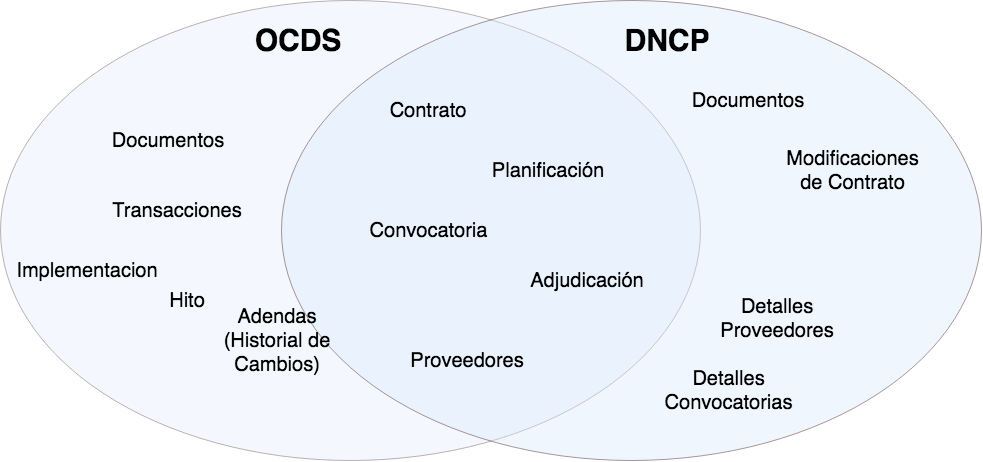
\includegraphics[width=150mm]{figuras/Diagramas-VennCobertura}
    \caption{Cobertura de los términos de la DNCP y la OCDS}
    \label{img:cobertura de la ontologia }
    \end{figure}

El OCDS es implementado a nivel internacional, tiene una comunidad de colaboradores expertos en el dominio de distintos países, implementadores que dan al estándar una validez en cuanto a la aceptación de los términos, posee listas de correos y un sistema de gestión de cambios y mejoras activo en la plataforma Github (https://github.com/open-contracting/standard). La intención de este trabajo es que la ontología sea utilizada no solamente por la DNCP sino por cualquier ente que realice procesos licitatorios, además, la DNCP está utilizando este estándar para publicación de datos orientados a desarrolladores. Con todo esto se aprecia que la cobertura es suficiente para utilizar el OCDS como recurso no-ontológico para nuestra ontología sacrificando así algunos detalles específicos de implementación local. Estos detalles más específicos se podrían cubrir a través del reuso y extensión de la ontología desarrollada en un futuro trabajo.

\section{Reingeniería de recurso no-ontológicos}
Debido a que se utilizó recursos no-ontológicos, debemos de realizar un proceso de reingeniería para transformar estos recursos de manera a incluir esa información en la ontología. Procedemos de esta manera al proceso de reingeniería del esquema de publicación de OCDS.

\subsection{Ingeniería reversa del recurso no-ontológico}
El primer paso es analizar el recurso no-ontológico para identificar los principales componentes y crear representaciones del recurso. Dentro de esta actividad procederemos a la recolección de los datos, la abstracción conceptual y exploración de la información.

\subsubsection{Recolección de datos}

El propósito de esta actividad es buscar y recolectar todos los datos y la documentación del recurso no-ontológico incluyendo su propósito, componentes, modelo de datos y detalles de implementación.

El OCDS es un estándar abierto de datos para la publicación de información estructurada sobre todas las etapas de un proceso de contratación: desde la planificación hasta la implementación.

La publicación de los datos siguiendo el OCDS permite una mayor transparencia en la contratación pública y puede apoyar al análisis accesible y a profundidad de la eficiencia, efectividad, equidad e integridad de los sistemas de contratación pública. El OCDS fue diseñado con un enfoque en la contratación pública de bienes, obras y servicios, pero puede ampliarse para su uso en otros contextos. 

El OCDS se centra en las siguientes necesidades del usuario:
\begin{itemize}
    \item Fortalecimiento de la transparencia, rendición de cuentas e integridad de los contratos públicos.
    \item Hacer un buen uso del dinero del gobierno.
    \item Permitir al sector privado una competencia justa por contratos públicos.
    \item Control de la eficacia de la prestación de servicios. 
\end{itemize}

El OCDS posee un sitio web donde se encuentra documentado todo el estándar, soportando los idiomas español, inglés y francés. Además posee una guía de implementación del estándar, un validador de la estructura sintáctica del mismo y un mecanismo de gestión de extensiones.

\subsubsection{Modelo conceptual}

En esta actividad se identifica el esquema de recursos así como también los componentes conceptuales y sus relaciones. Además se crea un modelo conceptual dividido por bloques de conceptos relacionados. El conocimiento se expresa mediante representaciones primitivas de conceptos y relaciones entre conceptos. A continuación se representa la conceptualización teniendo como base el OCDS.

Un proceso de contratación se define como toda la información relativa a la planificación, la licitación, las adjudicaciones, los contratos y la ejecución de contratos relacionados con un solo proceso de iniciación.

Un proceso de contratación agrupa información sobre diferentes etapas o fases relacionadas a la vida útil de un contrato, a partir de la planificación, progresando a través de las etapas de iniciación u oferta, luego por la adjudicación y contrato y finalizando con la implementación del producto o servicio como se muestra en la figura \ref{img:fases del proceso licitatorio }.

\begin{figure}[h!]
    \centering
    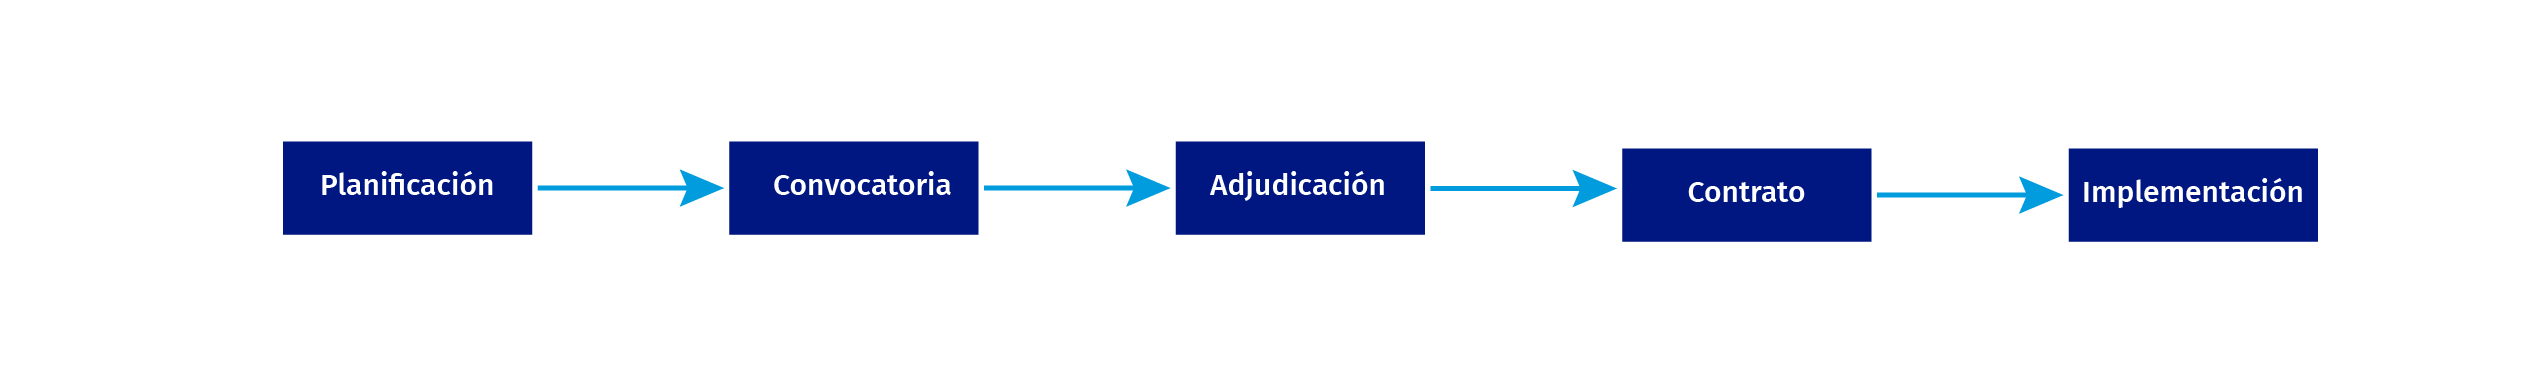
\includegraphics[width=150mm]{figuras/Diagramas_Mesa de trabajo 1 copia.png}
    \caption{Fases del Proceso Licitatorio}
    \label{img:fases del proceso licitatorio }
\end{figure}

Las etapas son correlativas, esto significa que necesariamente debe de existir la etapa anterior antes de existir la siguiente. Todas las etapas representan un bloque de información.

Además de estas etapas existe otro concepto importante que es el bloque de Organización, que puede corresponder tanto al comprador como al oferente. Esta Organización puede estar ligada a cualquiera de las etapas del proceso de contratación. A continuación se detallan cada una de las etapas.
\subsubsection{Planificación (Planning)}

Este bloque contiene información necesaria para describir los antecedentes de un proceso de contratación y puede incluir detalles del presupuesto del que se extraen los fondos o proyectos relacionados. Todo proceso de contratación posee una única planificación, dicha planificación tiene un presupuesto (budget) asociado donde finalmente se indica el valor o monto estimado para la adquisición del bien o servicio. Un diagrama de los componentes principales de la clase Planificación puede verse en la figura \ref{img:Fase de Planificacion}.

\begin{figure}[h!]
    \centering
    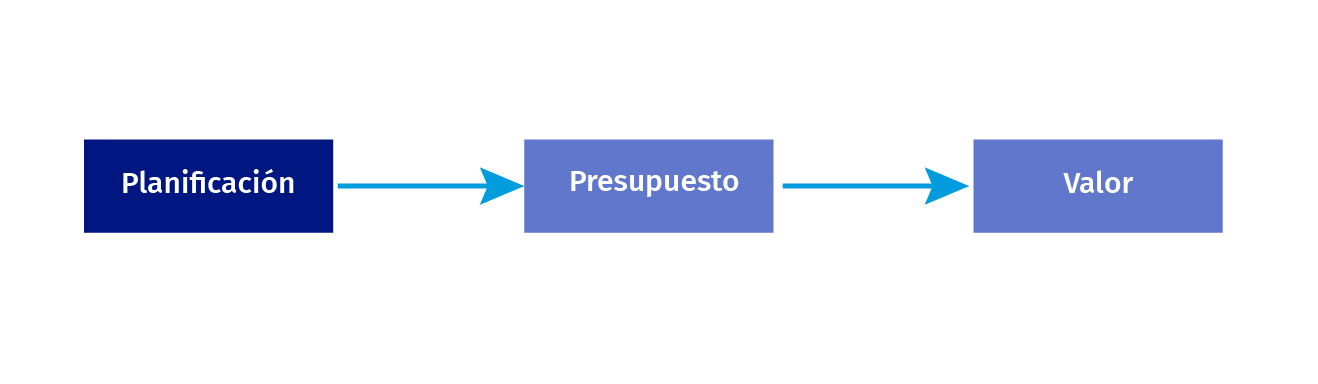
\includegraphics[width=150mm]{figuras/Diagramas_Mesa de trabajo 1.png}
    \caption{Fases del Proceso Licitatorio}
    \label{img:Fase de Planificacion}
\end{figure}